
%\subsection{Redes Neuronales}

\frame
{
  \frametitle{Neurona Biológica}
  \begin{columns}
  \column {0.5\textwidth}  
  En el cerebro humano hay aproximadamente ... %\pause  
  \begin{itemize}
  	\item 10 Billones de Neuronas  %\pause  
  	\item Cada neurona conectada a otras 10,000 neuronas %\pause  
  \end{itemize}
	Componentes: %%%%\pause    
  \begin{itemize}
  	\item Cuerpo de la Celula (SOMA) - Se puede entender como una unidad de procesamiento %\pause  
  	\item Axon - Salida %\pause  
  	\item Dentritas - Entradas %\pause  
  \end{itemize}

  \column {0.5\textwidth}  	
	  \begin{center}	  	
		  \begin{figure}      
			  %\pgfimage[height=3cm]{NeuronaBiologica}
			  \pgfimage[height=3cm]{Figs/NeuronaBiologicaV2} %\pause  
		  \end{figure}
		\end{center}  		
  \end{columns}
}



\frame
{
  \frametitle{Neurona Artificial}
  \begin{columns}
  \column {0.5\textwidth}  
  Surge como una imitación al modelo de neurona biológico   %\pause  
  \begin{itemize}
  	\item Entradas %\pause  
		\begin{itemize}
  		\item Patrones de entrada ($x_1...x_n$) %\pause  
  		\item Para cada entrada hay un peso asociado ($w_{1j} ... w_{nj}$) %\pause  
  	\end{itemize}
  	\item Componentes: %\pause  
		\begin{itemize}
  		\item función de transferencia - Generalmente es lineal.  %\pause  
  		\item función de activacion - Determinar cual es la salida de la Neurona. %\pause  
  	\end{itemize}	  	
  \end{itemize}
  \column {0.5\textwidth}  	
	  \begin{center}	  	
		  \begin{figure}      
			  \pgfimage[height=3cm]{Figs/NeuronaArtificial} %\pause  
		  \end{figure}	
		\end{center}  
  \end{columns}
}


\frame
{
\frametitle{Redes Neuronales}
\begin{itemize}  
	\item Las redes neuronales artificiales (RNA) son herramientas computacionales que resuelven una gran cantidad de problemas: 
		\begin{itemize}
			\item Diagnóstico médico %\pause  
			\item Procesamiento de Im\'agenes %\pause  
			\item Control Robótico %\pause  
		\end{itemize}
	\item Las RNA estan inspiradas biológicamente pero  %\pause  
		\begin{itemize}
		\item Requieren de una gran cantidad de operaciones  %\pause  
		\item Las computadoras actuales no son adecuadas para su implementación %\pause  
		\end{itemize}
	\item Hay avances significativos en cuanto a circuitos de alta velocidad %\pause  
		\begin{itemize}
		\item Debido a la amplia disponibilidad de tarjetas gráficas con unidades de procesamiento gráficos (GPUs), es posible utilizar redes con un desempeño aceptable
		\item En tiempos recientes, incluso los dispositivos móviles tienen incorporados unidades especiales conocidas como Neural Processing Unit (NPUs), además de los GPUs
		\end{itemize}
\end{itemize}
}

\frame
{
  \frametitle{Generaciones de RNAs \cite{WANG2020258}}
  \begin{columns}
  \column {0.5\textwidth} 
  \begin{enumerate}
 \item Utilizan neuronas McCulloch-Pitts como unidades computacionales, cuyo valor de salida es una variable binaria. 
 \item Utilizan unidades computacionales con una función de activación continua para realizar el procesamiento de la entrada y salida numérica real.
 \item Utilizan neuronas con picos biológicamente plausibles como unidades computacionales básicas.
  \end{enumerate}
   
%\cite{7929186}

  \column {0.5\textwidth}  	
    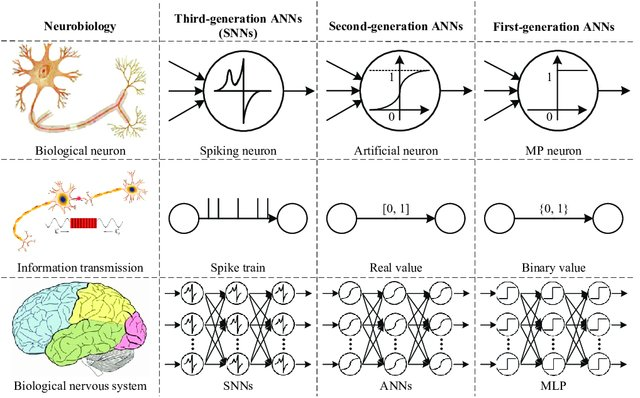
\includegraphics[width=\textwidth]{Figs/GeneracionesRNAs}	
  \end{columns}
%\footnotetext[1]{https://towardsdatascience.com/the-mostly-complete-chart-of-neural-networks-explained-3fb6f2367464}
}



\begin{frame}{Aprendizaje Máquina vs Aprendizaje Profundo}
%\Huge

	%\begin{block}{Aprendizaje Máquina} 
		\begin{columns}
		\begin{column}{0.57\textwidth}
		\begin{block}{Aprendizaje Máquina} 
		\begin{itemize}
		\item Existen varios algoritmos, uno de los más utilizados son las Redes Neuronales.
		\end{itemize}
		\end{block} 
        \begin{block}{Aprendizaje Profundo} 
		\begin{itemize}
		\item La red neuronal convolucional es una subclase de redes neuronales que tienen al menos una capa de convolución. 
        \item Capturan información local y reducen la complejidad del modelo.
%		\item Una generación de algoritmos que permiten resolver tareas.
		%\item Las computadoras intentan resolver tareas que solo son posibles mediante inteligencia humana
		%\item Es una rama muy amplia que cubre muchos aspectos de la vida cotidiana.
		\end{itemize}
		\end{block} 

		\end{column}
		\begin{column}{0.37\textwidth}  
			\begin{center}
			 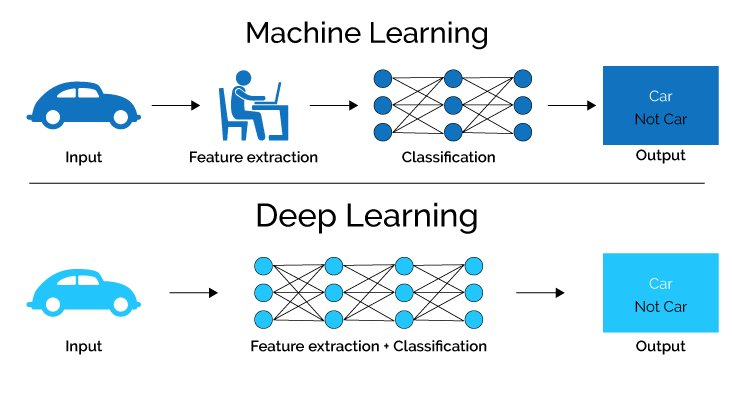
\includegraphics[width=\textwidth]{Figs/MachineLearningVsDeepLearning}
			 %\includegraphics[width=\textwidth]{WordReading2}
			 \end{center}
		\end{column}
	\end{columns}
	%\end{block} 
\end{frame}

\frame
{
  \frametitle{Tipos de RNAs}
  \begin{columns}
  \column {0.5\textwidth}  
    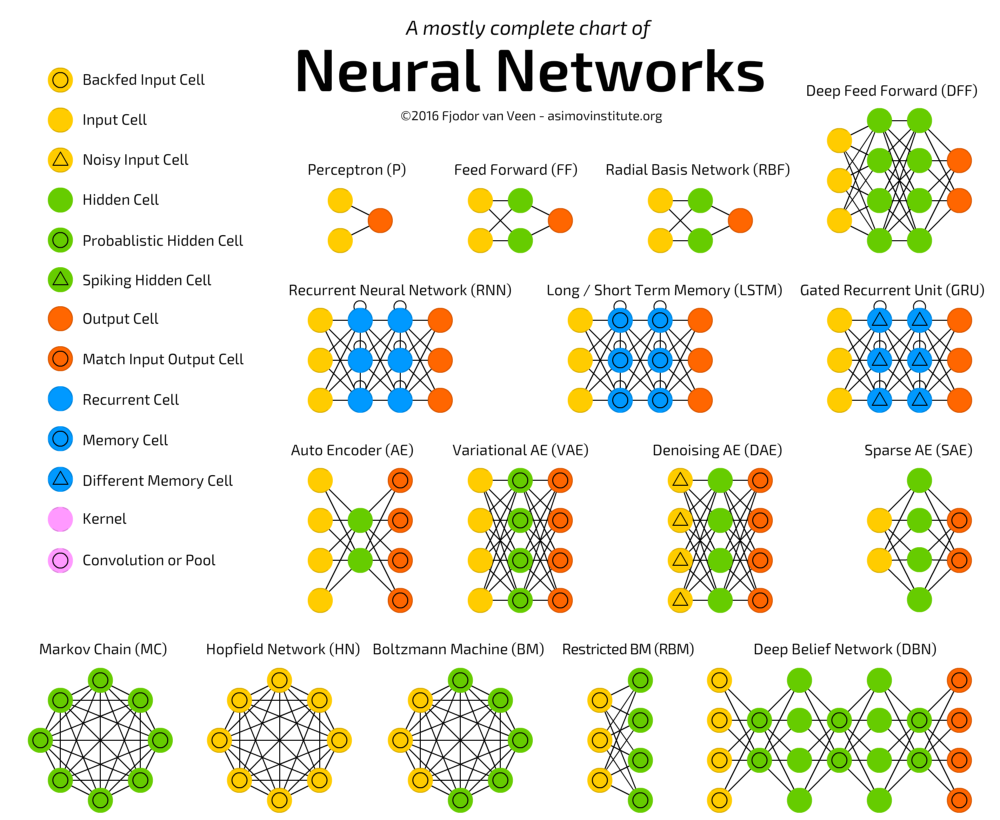
\includegraphics[width=\textwidth]{Figs/AMostlyNN_01}
  \column {0.5\textwidth}  	
    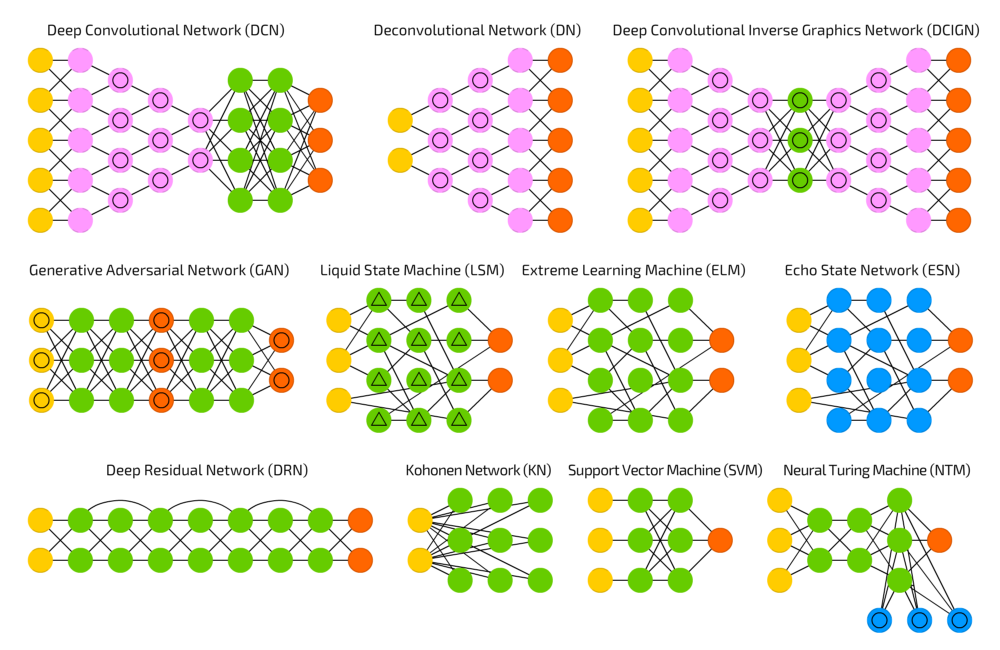
\includegraphics[width=\textwidth]{Figs/AMostlyNN_02}	
  \end{columns}
\footnotetext[1]{https://towardsdatascience.com/the-mostly-complete-chart-of-neural-networks-explained-3fb6f2367464}
}



